\section{Results}
% * <mmore500.login@gmail.com> 2017-12-13T20:06:31.427Z:
%
% ^.

\begin{figure}
    \centering
    \begin{subfigure}[t]{0.5\columnwidth}
        \centering
        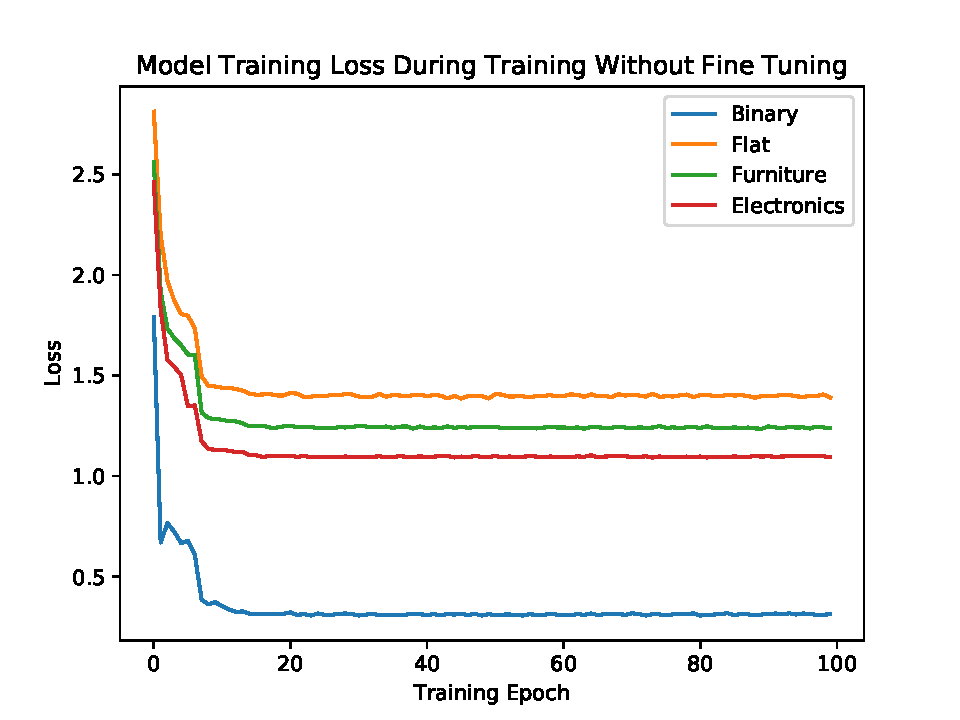
\includegraphics[width=\textwidth]{img/false_losses_train}
        \caption{}
    \end{subfigure}%
    ~ 
    \begin{subfigure}[t]{0.5\columnwidth}
        \centering
        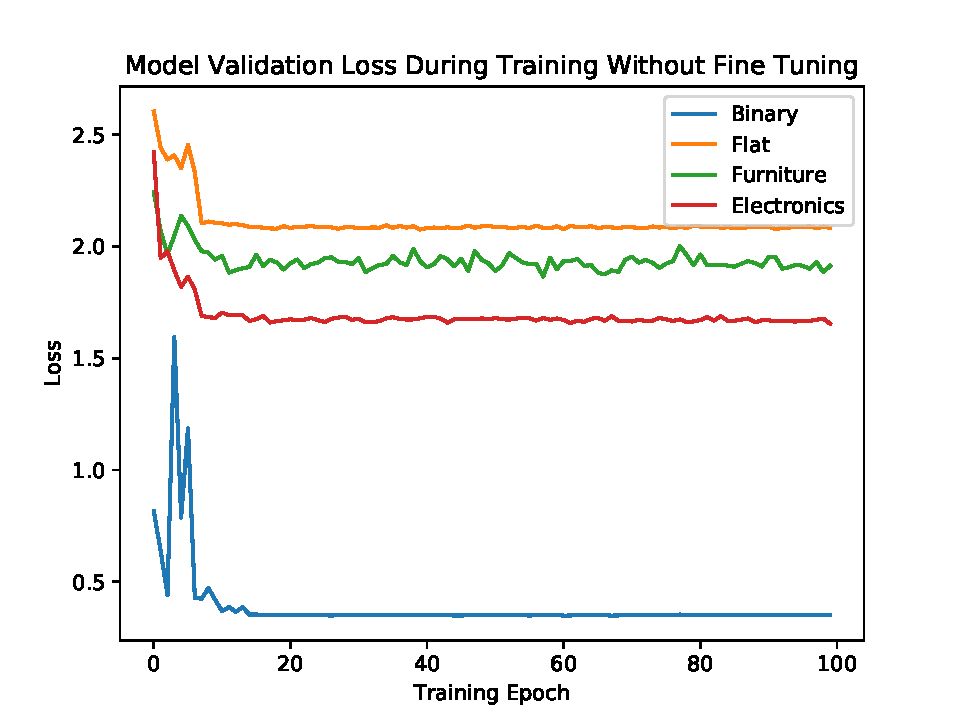
\includegraphics[width=\textwidth]{img/false_losses_val}
        \caption{}
    \end{subfigure}%
	\caption{
Loss values of our models during training without fine tuning.
Subfigure (a) displays training loss by epoch.
Subfigure (b) displays testing loss by epoch. 
}
	\label{fig:false_losses}
\end{figure}
\begin{figure}
    \centering
    \begin{subfigure}[t]{0.5\columnwidth}
        \centering
        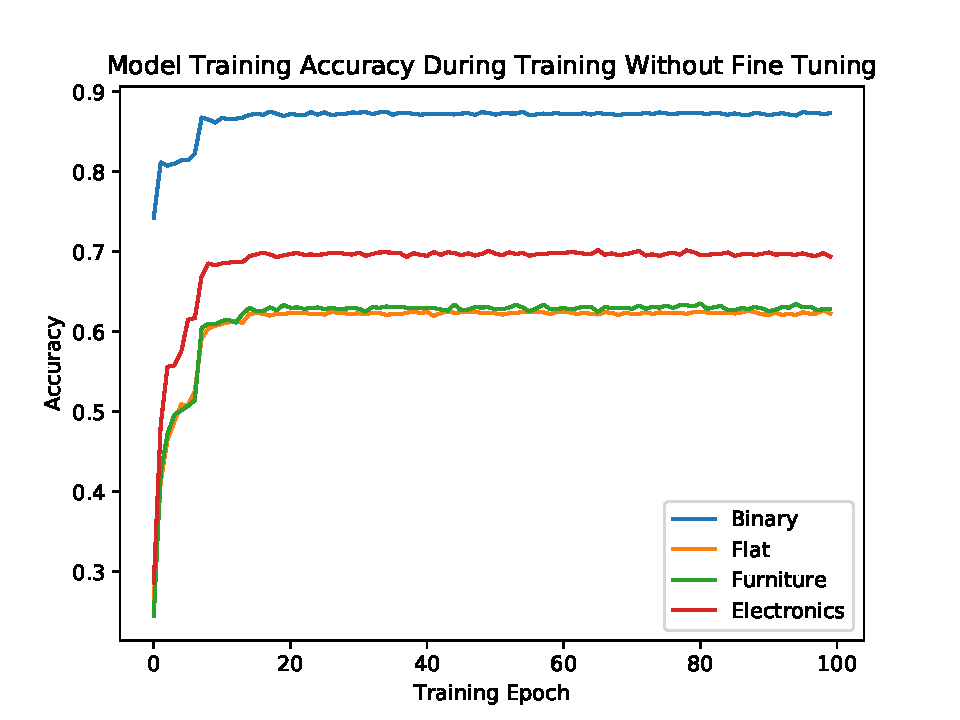
\includegraphics[width=\textwidth]{img/false_accs_train}
        \caption{}
    \end{subfigure}%
    ~ 
    \begin{subfigure}[t]{0.5\columnwidth}
        \centering
        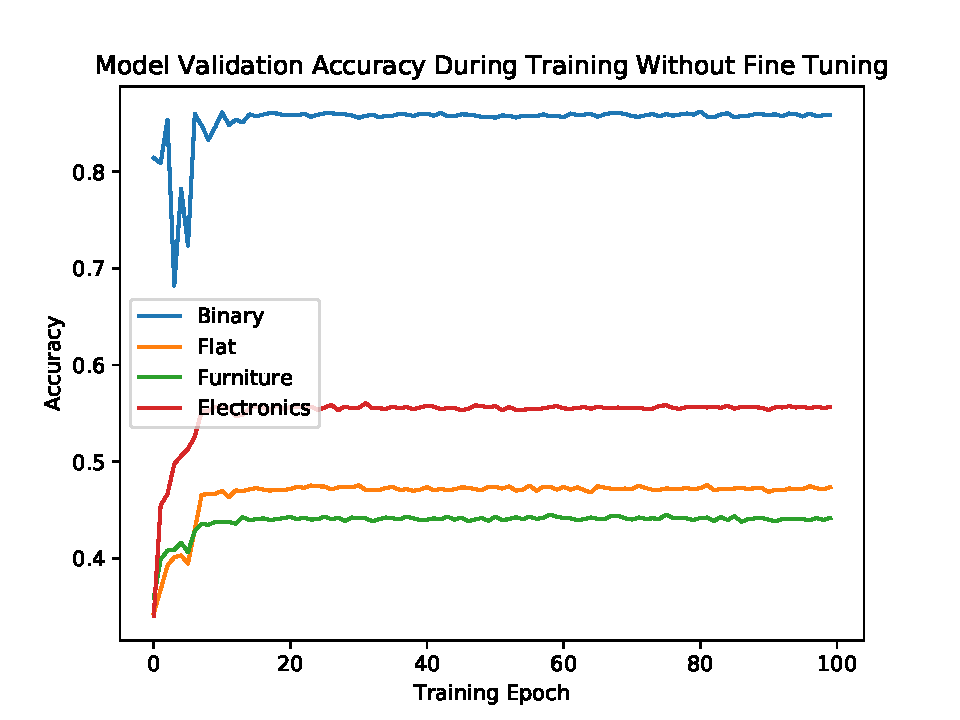
\includegraphics[width=\textwidth]{img/false_accs_val}
        \caption{}
    \end{subfigure}%
	\caption{
Classification accuracy of our models during training without fine tuning.
Subfigure (a) displays training accuracy by epoch.
Subfigure (b) displays testing accuracy by epoch. 
}
	\label{fig:false_accs}
\end{figure}
\begin{figure}
    \centering
    \begin{subfigure}[t]{0.5\columnwidth}
        \centering
        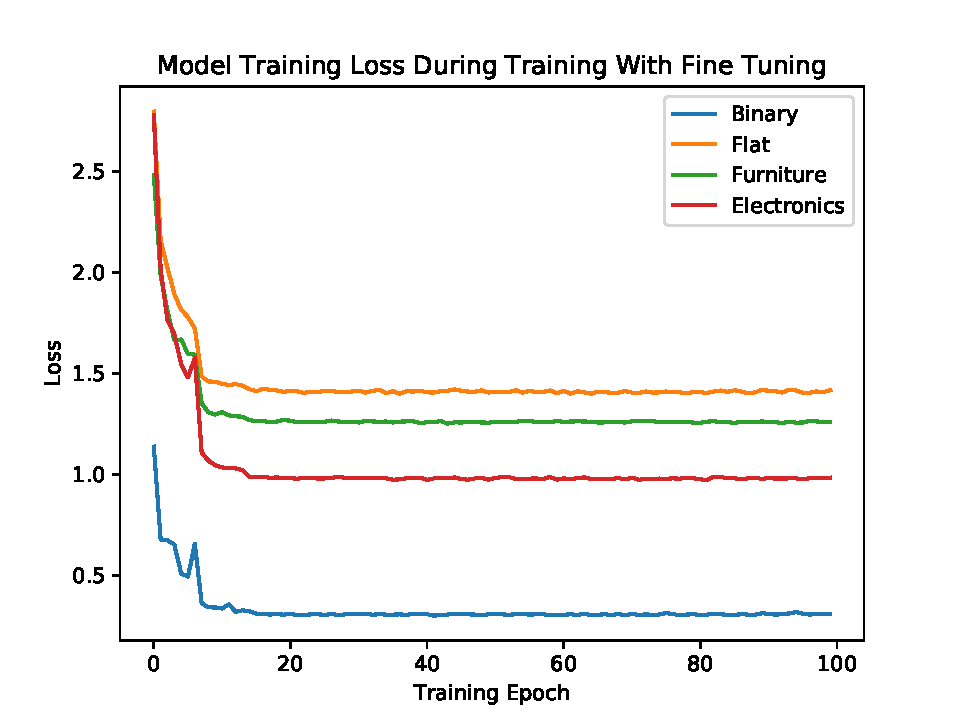
\includegraphics[width=\textwidth]{img/true_losses_train}
        \caption{}
    \end{subfigure}%
    ~ 
    \begin{subfigure}[t]{0.5\columnwidth}
        \centering
        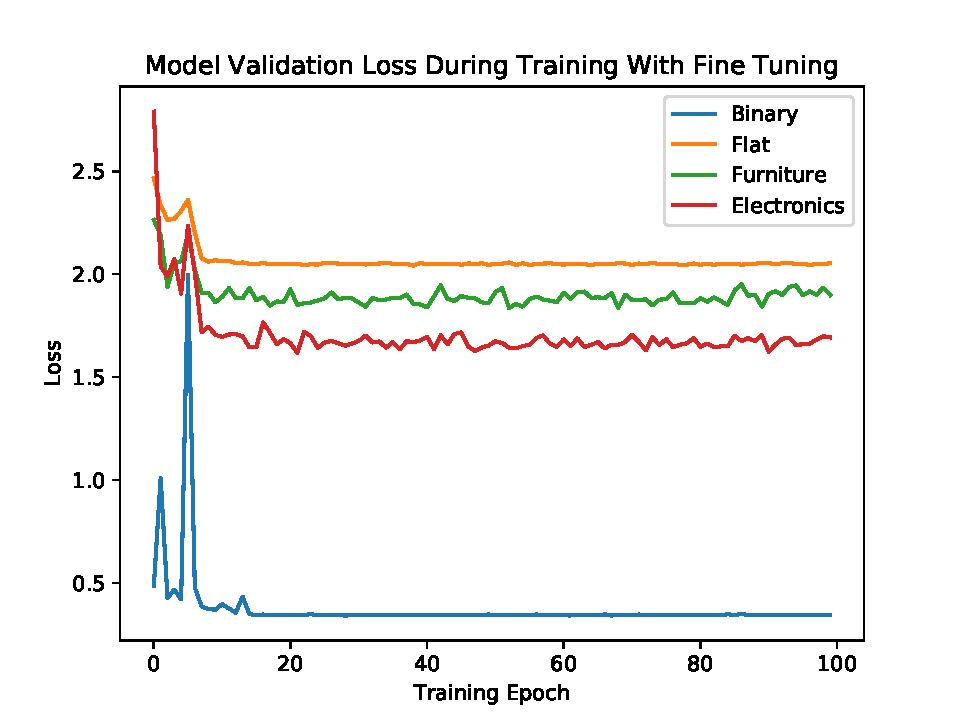
\includegraphics[width=\textwidth]{img/true_losses_val}
        \caption{}
    \end{subfigure}%
	\caption{
Loss values of our models during training with fine tuning.
Subfigure (a) displays training loss by epoch.
Subfigure (b) displays testing loss by epoch. 
}
\label{fig:true_losses}
\end{figure}
\begin{figure}
    \centering
    \begin{subfigure}[t]{0.5\columnwidth}
        \centering
        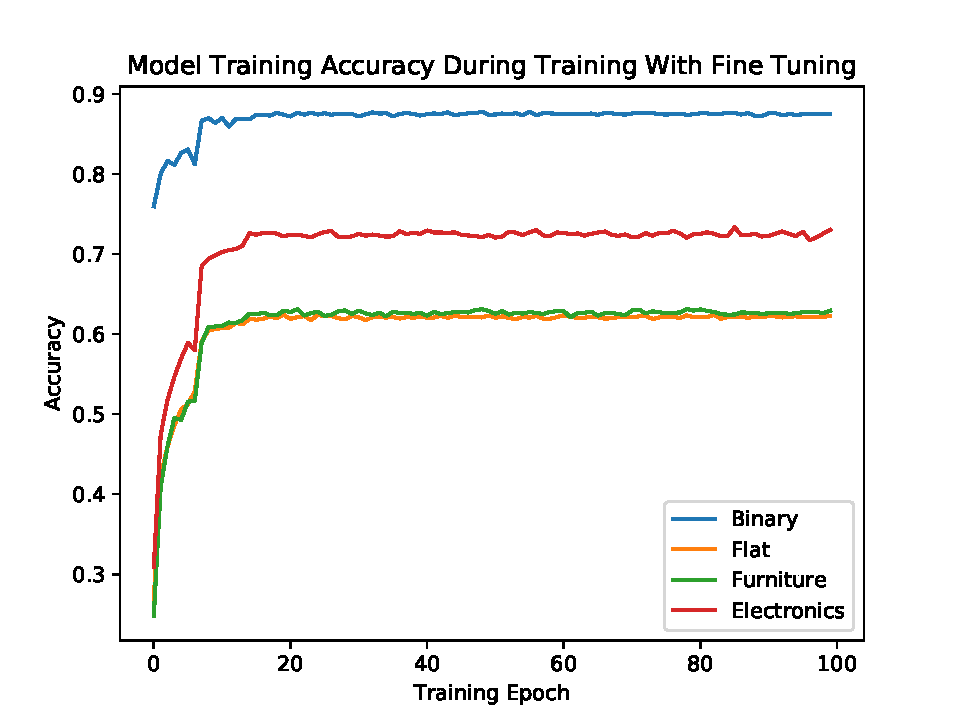
\includegraphics[width=\textwidth]{img/true_accs_train}
        \caption{}
    \end{subfigure}%
    ~ 
    \begin{subfigure}[t]{0.5\columnwidth}
        \centering
        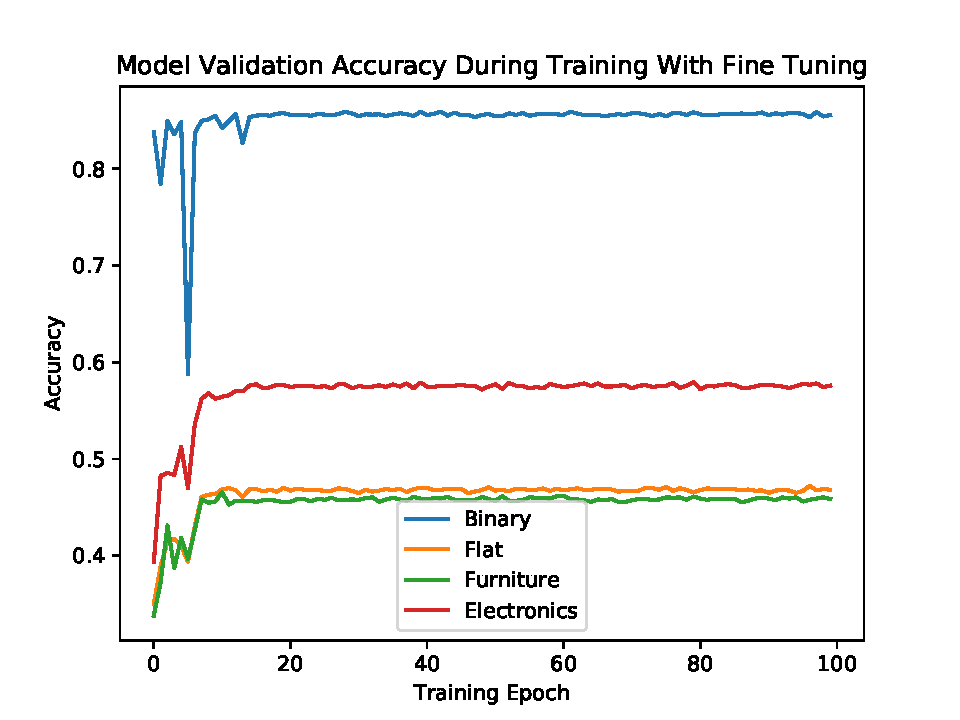
\includegraphics[width=\textwidth]{img/true_accs_val}
        \caption{}
    \end{subfigure}%
	\caption{
Classification accuracy of our models during training with fine tuning.
Subfigure (a) displays training accuracy by epoch.
Subfigure (b) displays testing accuracy by epoch. 
}
	\label{fig:true_accs}
\end{figure}
\begin{figure}
\begin{center}
\begin{tabular}{ c|c c } 
 ~ & Flat & Hierarchical \\
 \hline
 fine tuning & 0.5813 & 0.4076 \\ 
 no fine tuning & 0.5891 & 0.5540 \\ 
\end{tabular}
\end{center}
\caption{
Validation set classification accuracy of flat model and hierarchical models approaches with and without fine tuning.
}
\label{fig:acc_table}
\end{figure}

Figures \ref{fig:false_losses} and \ref{fig:true_losses} show training and testing loss by epoch for the four ResNet models that were trained (three for the hierarchical models approach, one for the flat model approach). 
Specifically, Figure \ref{fig:false_losses} documents loss by epoch for transfer learning without fine tuning and Figure \ref{fig:true_losses} documents loss by epoch for transfer learning with fine tuning.
In both cases, testing loss exceeds training loss to some extent for the flat, furniture, and electronics models, indicating that these models overfit the training data.
Based on the difference between training and testing loss, the extent of overfitting appears to be comparable both with and without fine tuning.
However, training and testing loss was very similar for the binary classification model both with and without fine tuning, suggesting this model did not as strongly overfit its training data.
Perhaps this reduced overfitting was due to a greater number of training examples being available per class because this model only catergorizes between two classes.

Figures \ref{fig:false_accs} and \ref{fig:true_accs} show training and testing classification accuracy by epoch for the four ResNet models that were trained.
Specifically, Figure \ref{fig:false_accs} shows classification accuracy by epoch for transfer learning without fine tuning and Figure \ref{fig:true_accs} shows classification accuracy by epoch for transfer learning with fine tuning.
In both cases, training accuracy significantly exceeds training accuracy for the flat, furniture, and electronics models, providing another indication that these models overfit the training data. 
As before, testing and training accuracies were more similar for the binary classification model with and without fine tuning, suggesting that this model did not as strongly overfit its training data.
Interestingly, the both with and without fine tuning testing classification accuracy for the electronics model significantly exceeded the testing classification accuracy for the furniture model, suggesting that discriminating between low-level furniture classes was a more difficult problem for our methods than discriminating between low-level electronics classes.
In fact, both with and without fine tuning classification accuracy for the furniture model was similar to that of the furniture model, even though the flat model must categorize between twice as many categories.
In some cases classification accuracy for the flat model seems to actually slightly exceed the classification accuracy for the furniture model.
The poor performance of the furniture-only classifier relative to the electronics-only classifier may be an artifact of the particular low-level furniture classes that we included in our reduced dataset or simply of the furniture low-level classes in general.
However, the sometimes slightly superior classification accuracy of the flat model is perplexing because the flat model must in fact perform the same furniture classifications as the furniture-only model.

Finally, Figure \ref{fig:acc_table} summarizes the classification accuracies of the flat model approach and the hierarchical models approach.
The flat model approach yielded better classification accuracy than the hierarchical models approach, both with and without fine tuning.
The hierarchical model performed somewhat comparably to the flat model without fine tuning but its classification accuracy suffered significantly when fine tuning was used while training its constituent models.